\chapter{Results and Discussions}
\label{chap:experiments_and_results}

\section{Prototype Implementation Status}
The repository contains a working full-stack prototype, not just an architecture proposal. A user can register and sign in, submit context through an authenticated API, and review a response in the dashboard. Requests are persisted, and the separate agent service registers nine specialists that the root agent can select through its routing instructions. The source also includes GitHub diff retrieval, Jira Cloud OAuth and issue retrieval, and optional Microsoft Entra authentication.

\begin{table}[htbp]
\centering
\small
\begin{tabularx}{\textwidth}{p{0.30\textwidth}p{0.20\textwidth}X}
\toprule
\textbf{Project area} & \textbf{Status in inspected repository} & \textbf{Evidence or qualification} \\
\midrule
Problem analysis and architecture & Implemented & Research framing is documented in the proposal and presentation; current services are separated into frontend, backend, and agent. \\
Core quality-assistance flow & Implemented & Authenticated request persistence, prompt construction, agent call, and response persistence are present. \\
Specialist STLC capabilities & Implemented & Nine task-focused agents are registered; orchestration is controlled by ADK and agent instructions. \\
Jira and GitHub context & Implemented, configuration-dependent & OAuth and issue retrieval are available for Jira; GitHub repository settings support diff retrieval. \\
Authentication and deployment controls & Implemented in part & Password/JWT authentication, optional Entra SSO, encrypted integration credentials, and production settings validation are present. \\
RAG over organizational test assets & Planned & No persistent requirements/test/defect retrieval index is evidenced in the inspected implementation. \\
Automated CI test execution and script mutation & Planned / out of scope of current behavior & Execution and healing agents analyze or recommend; they do not execute external suites or commit changes. \\
Comparative empirical evaluation & Pending & No measured baseline, benchmark results, or controlled organizational pilot results were supplied. \\
\bottomrule
\end{tabularx}
\caption{Implementation status as of November 2026, distinguishing current behavior from planned work.}
\label{tab:implementation-status}
\end{table}

\section{Existing Automated Test Assets}
Focused test modules cover Bedrock credential settings, backend production configuration, Jira Cloud service behavior, and Microsoft Entra SSO behavior. These tests show that selected configuration and integration paths have dedicated checks. They do not establish that the tests pass, nor do they validate every UI, model, database, or agent workflow end to end. A reproducible submission should include the command, environment, commit, test count, and outcome from an actual run.

\section{Demonstration Scenarios}
The dashboard includes sample inputs that can be used to demonstrate several agent routes:
\begin{enumerate}
  \item a password-reset requirement for test planning and requirement summarization;
  \item an e-commerce checkout scenario with requirements, user stories, and a code diff;
  \item a diff-heavy authentication change for regression impact analysis;
  \item a test-run log containing pass, fail, and skipped cases for execution analysis and reporting;
  \item a Playwright selector change for automation and self-healing recommendations; and
  \item a follow-up request that reuses the prior session identifier.
\end{enumerate}
These examples show that the interface and request model can handle several kinds of context. They are demonstrations, not a benchmark, and provide no measurement of coverage, effort, or defect detection.

\subsection{Interface Walkthrough and Illustrative Outputs}
The screenshots follow a typical request: opening the workspace, checking integration settings, entering requirements and a user story, then reviewing the response. They document the interface and sample output only. No controlled evaluation was performed, and recommendations shown here still need human review.

\begin{figure}[H]
\centering
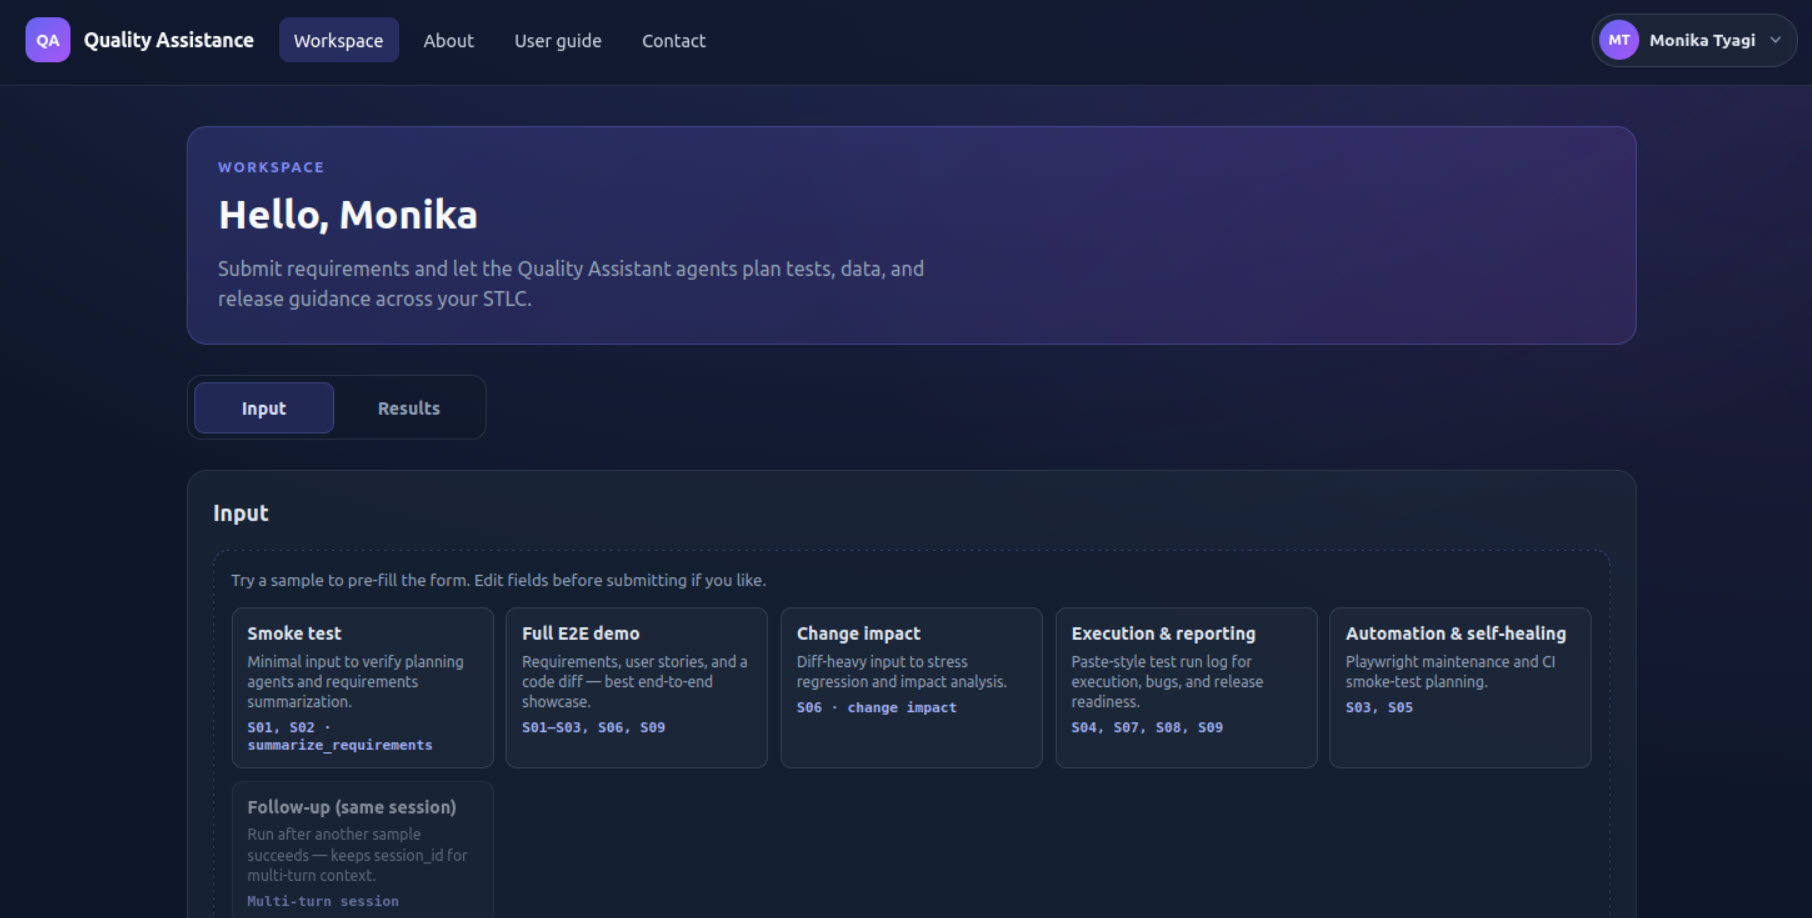
\includegraphics[width=\textwidth,height=0.46\textheight,keepaspectratio]{home.jpg}
\caption{Workspace dashboard used to start a quality-assistance request.}
\label{fig:workspace-dashboard}
\end{figure}

\begin{figure}[H]
\centering
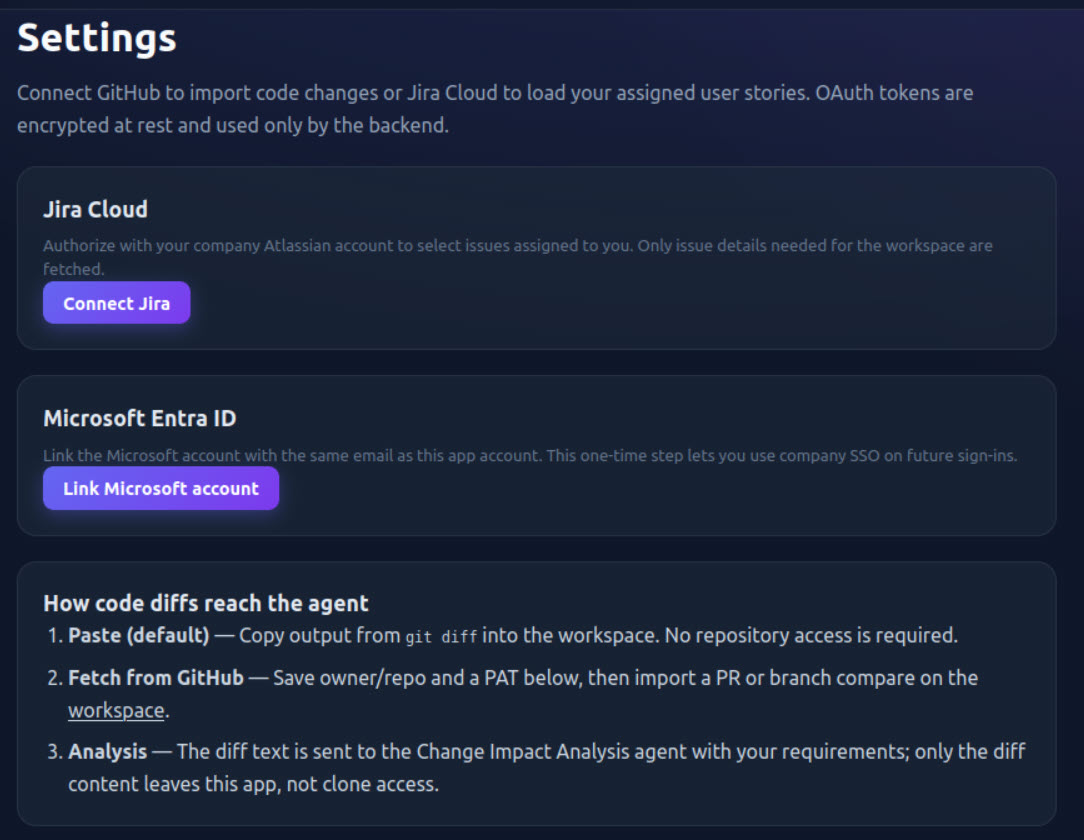
\includegraphics[width=0.9\textwidth,height=0.46\textheight,keepaspectratio]{settings.jpg}
\caption{Settings page for configuring Jira, GitHub, and sign-in integrations. Availability depends on administrator configuration and valid credentials.}
\label{fig:integration-settings}
\end{figure}

\begin{figure}[H]
\centering
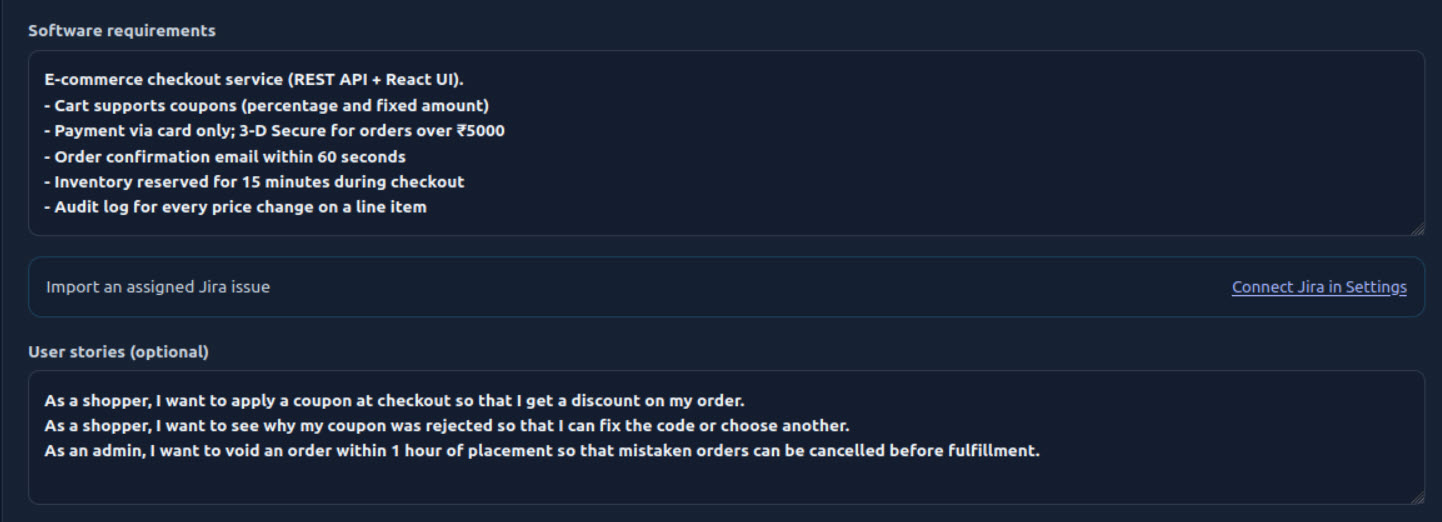
\includegraphics[width=\textwidth,height=0.42\textheight,keepaspectratio]{input.jpg}
\caption{Example request input containing quality context and a user story before agent processing.}
\label{fig:request-input}
\end{figure}

\begin{figure}[H]
\centering
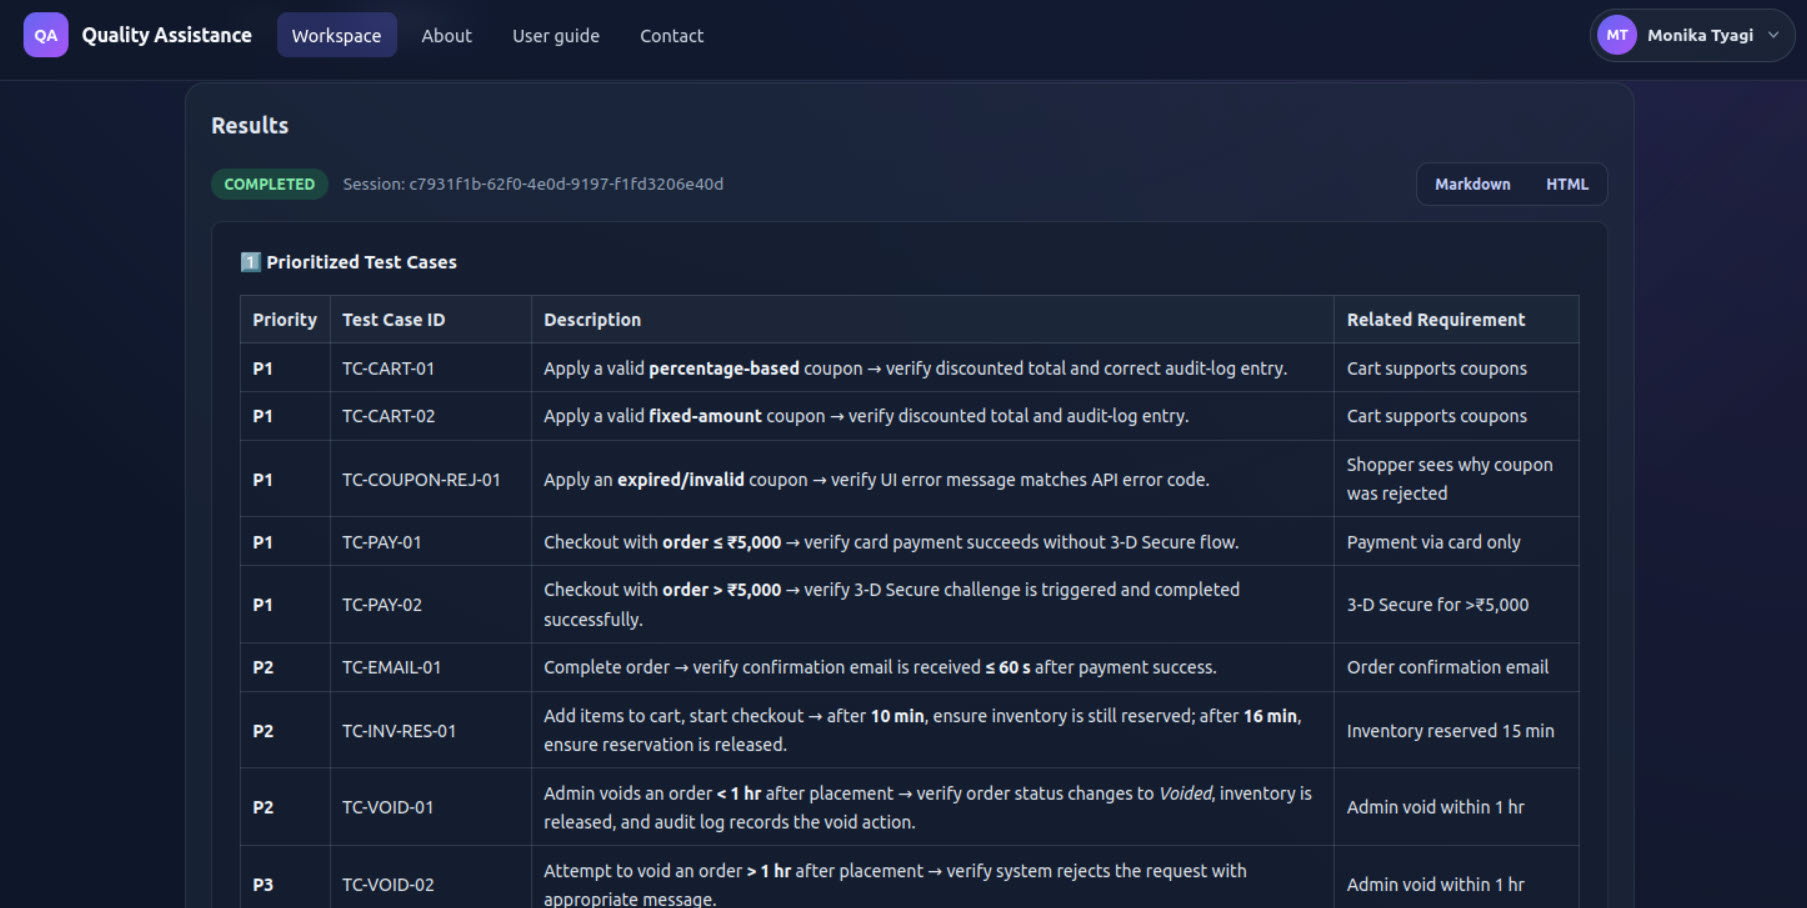
\includegraphics[width=\textwidth,height=0.46\textheight,keepaspectratio]{result.jpg}
\caption{Example generated response with prioritized test-case recommendations.}
\label{fig:prioritized-results}
\end{figure}

\begin{figure}[H]
\centering
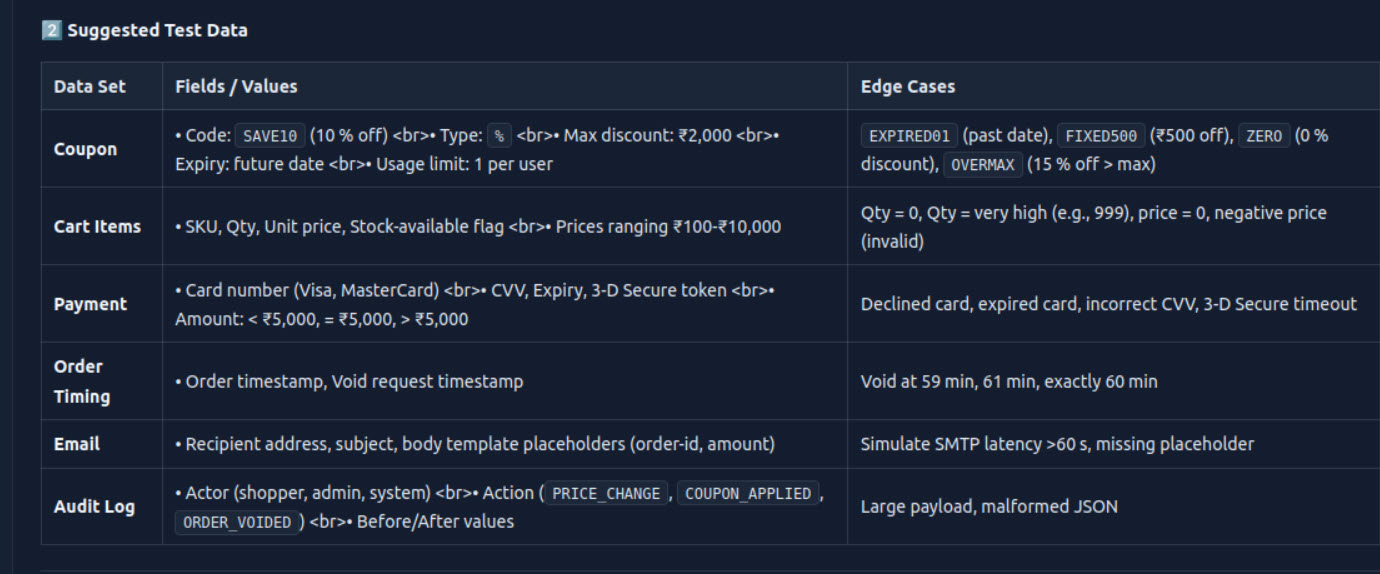
\includegraphics[width=\textwidth,height=0.42\textheight,keepaspectratio]{result2.jpg}
\caption{Example suggested test data presented as part of the generated response.}
\label{fig:suggested-test-data}
\end{figure}

\begin{figure}[H]
\centering
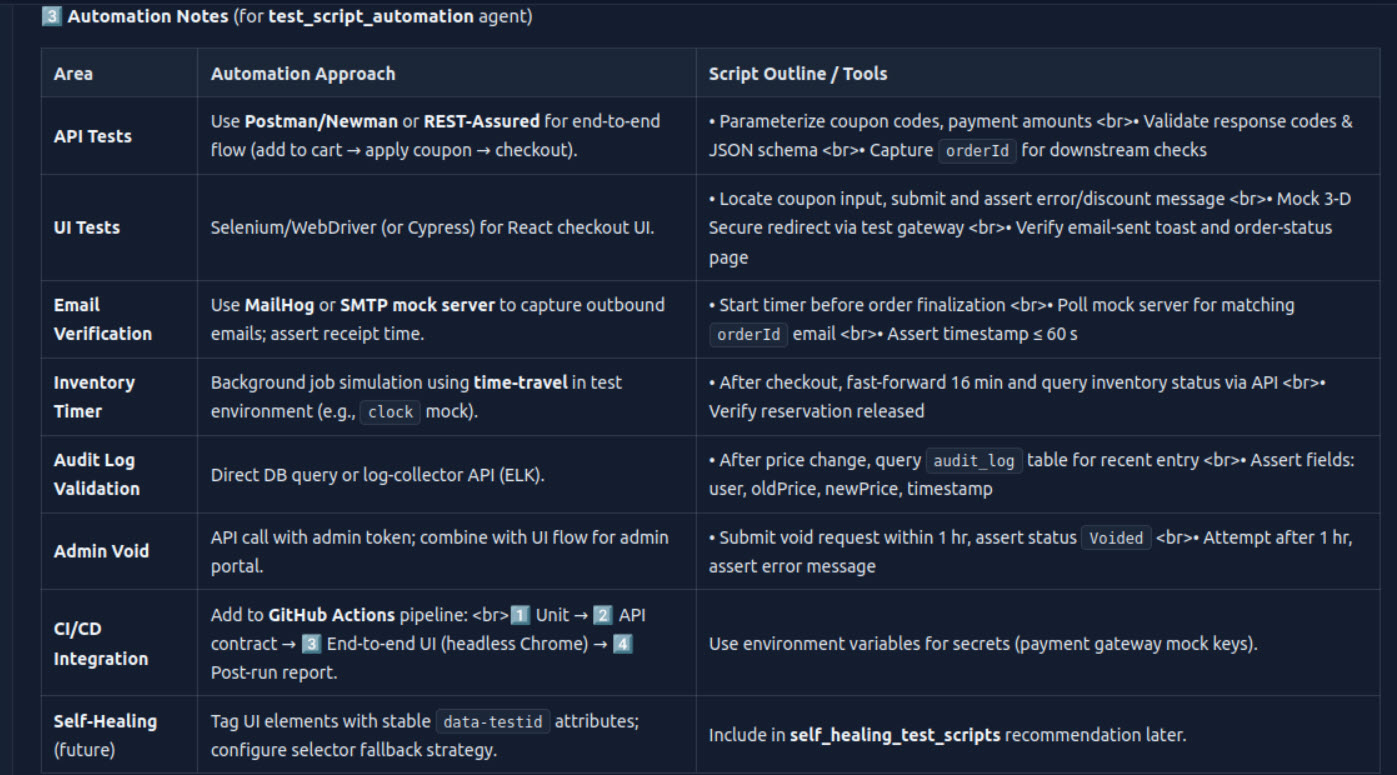
\includegraphics[width=\textwidth,height=0.46\textheight,keepaspectratio]{result3.jpg}
\caption{Example automation notes and test-script recommendations.}
\label{fig:automation-results}
\end{figure}

\begin{figure}[H]
\centering
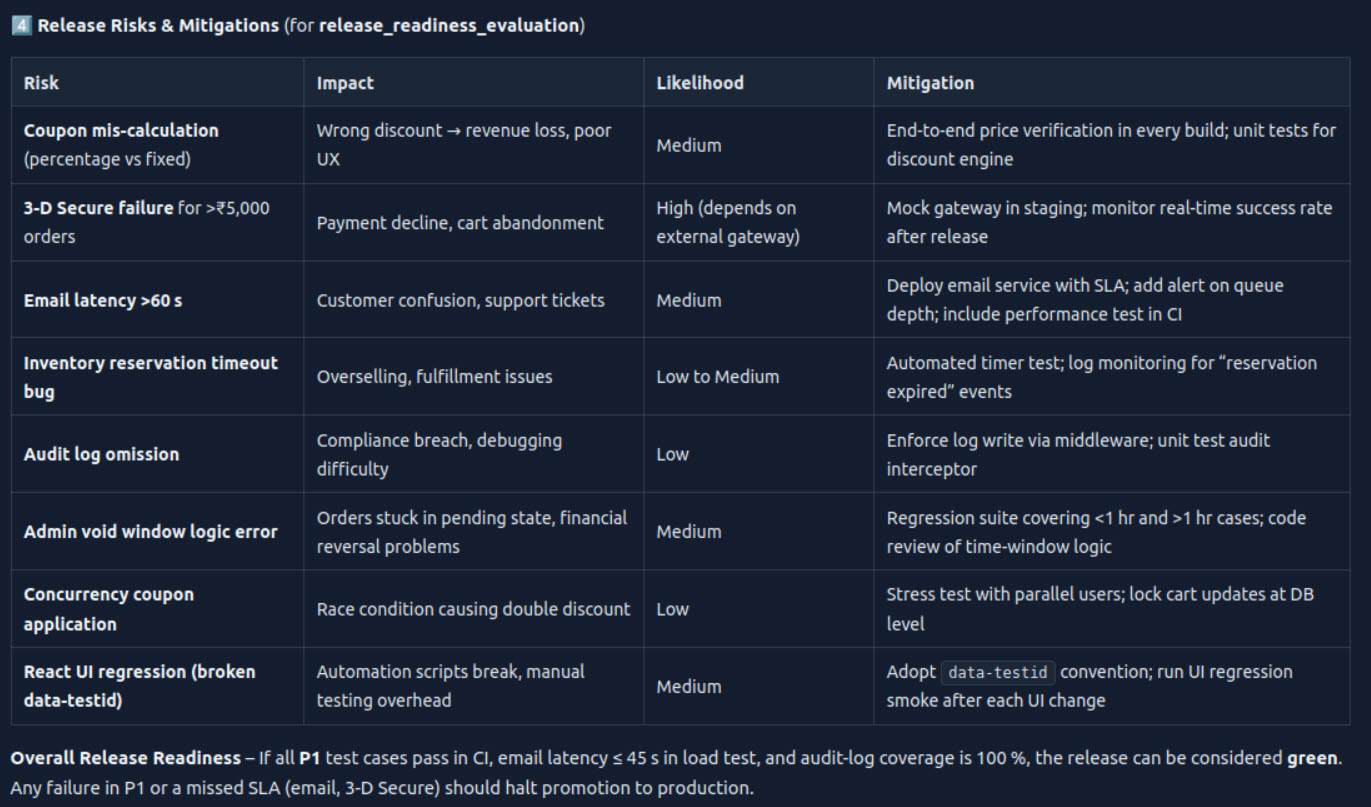
\includegraphics[width=\textwidth,height=0.46\textheight,keepaspectratio]{result4.jpg}
\caption{Example release-risk and readiness analysis based on the submitted context.}
\label{fig:readiness-results}
\end{figure}

\section{Evaluation Plan}
The evaluation should compare three conditions on the same tasks: a manual QA baseline, an existing point-automation workflow where available, and the proposed assistant-supported workflow. The initial phase should use public requirements and open-source repositories or issue trackers, as proposed in the project plan. Any later organizational evaluation should use anonymized artifacts and receive the required data-governance approval.

\subsection{Dataset and Protocol}
For each project, select a bounded set of requirements, user stories, code changes, and available test-run or defect records. Define expected requirement-to-test links and expert-reviewed reference outputs before running the assistant. Use a fixed model, model version, prompt revision, and application configuration for each comparison. Because model outputs can vary, repeat tasks where practical and retain both raw outputs and review decisions. The reviewer should be blind to the workflow condition when rating generated artifacts, where feasible.

\subsection{Measures}
\begin{table}[htbp]
\centering
\small
\begin{tabularx}{\textwidth}{p{0.25\textwidth}p{0.31\textwidth}X}
\toprule
\textbf{Measure} & \textbf{Operational definition} & \textbf{Interpretation} \\
\midrule
Requirement traceability & Percentage of in-scope requirements linked to at least one reviewer-accepted test case. & Tests whether generated artifacts preserve requirement coverage links. \\
Scenario coverage & Reviewer-rated coverage of agreed positive, negative, boundary, and risk conditions. & Measures breadth and relevance rather than the raw number of generated cases. \\
Artifact correctness & Proportion of sampled cases judged correct and actionable by independent reviewers. & Captures factual and procedural quality; report agreement between reviewers. \\
Effort & Active authoring and review time per requirement or change. & A reduction is meaningful only if review and correction time are included. \\
Defect analysis quality & Precision, recall, or F-score against adjudicated defect categories when labels exist. & Applies only where a suitable labeled reference set is available. \\
Response time and cost & End-to-end latency and model usage per completed task. & Quantifies operational overhead and helps assess scalability. \\
User acceptance & Structured ratings of usefulness, clarity, and trust from representative practitioners. & Complements objective measures but should not replace correctness review. \\
\bottomrule
\end{tabularx}
\caption{Proposed evaluation measures; no values are reported because a controlled evaluation has not yet been completed.}
\label{tab:evaluation-metrics}
\end{table}

\subsection{Analysis and Validity}
For quantitative comparisons, report sample sizes, distributions, confidence intervals, and the selected statistical tests. Analyze error categories as well as aggregate scores. Conduct qualitative review of omissions, unsupported statements, ambiguous requirements, and cases where the model's recommendation conflicts with expert judgment. Record the model and prompt versions so that repeated evaluations remain interpretable.

Threats to validity include dataset representativeness, evaluator subjectivity, model nondeterminism, changes in external model services, contamination between task examples and prompts, and the possibility that generated cases increase review burden. A small public-data evaluation would support feasibility claims but would not alone establish generalization to enterprise workflows.

\section{Results and Discussion}
The evidence available here is implementation evidence. The application accepts quality context, stores a request, calls the orchestrated agent, and returns a response. Its specialist registry and dashboard examples cover several STLC tasks, while the integration code provides a starting point for connecting engineering systems.

The materials reviewed for this report did not include experiment results, a benchmark dataset, measured time savings, coverage figures, defect-detection rates, or user-study findings. It is therefore not possible to claim that the system improves quality or reduces effort. The result at this stage is the software artifact and a protocol for testing those claims. Plausible-looking generated cases are not, on their own, evidence that the cases are complete, correct, or effective at finding defects.

\section{Limitations}
\begin{itemize}
  \item The quality of recommendations depends on the completeness and accuracy of user-supplied context and the selected model.
  \item Cross-agent routing and synthesis are predominantly prompt-driven; formal inter-stage schemas and independent quality gates are not evidenced.
  \item Agent session state uses an in-memory runner and is not a durable conversation store across process restarts.
  \item The system does not autonomously execute external test suites, modify scripts, or enforce release approvals.
  \item Persistent retrieval over requirements, test assets, and historical defects and a Jenkins or equivalent CI/CD integration are future work.
  \item The available repository tests address selected settings and service behavior; comprehensive user-interface, model-quality, load, and end-to-end tests remain necessary.
  \item Production deployment and organization-specific security and privacy approval are not demonstrated by the deployment planning documents.
\end{itemize}
